
%----------------------------------------------------------------------------------------
%	PACKAGES AND DOCUMENT CONFIGURATIONS
%----------------------------------------------------------------------------------------

\documentclass{article}

\usepackage[version=3]{mhchem} % Package for chemical equation typesetting
\usepackage{siunitx} % Provides the \SI{}{} and \si{} command for typesetting SI units
\usepackage{graphicx} % Required for the inclusion of images
\usepackage{natbib} % Required to change bibliography style to APA
\usepackage{amsmath} % Required for some math elements 
\usepackage{amssymb}
\setlength\parindent{0pt} % Removes all indentation from paragraphs
\usepackage{hyperref}
\renewcommand{\labelenumi}{\alph{enumi}.} % Make numbering in the enumerate environment by letter rather than number (e.g. section 6)
\usepackage{xfrac}
%\usepackage{times} % Uncomment to use the Times New Roman font
\usepackage{nicefrac}
\usepackage{graphicx}
\usepackage{caption}
\usepackage{subcaption}
%----------------------------------------------------------------------------------------
%	DOCUMENT INFORMATION
%----------------------------------------------------------------------------------------

\title{Graphic User Interface \\ User Guide \\ Version 1.0} % Title

\author{Haoran \textsc{Yu}} % Author name

\date{4/8/2016} % Date for the report

\begin{document}

\maketitle

This document is the User Guide for Matlab generated Graphic User Interface. This document will include three sections.
\begin{enumerate}
\item Introduction: introduce the interface and detail steps for use. Arm 2 is always the camera arm.
\item Arm setup: with estimate clinical setup. How to get actual setup.
\item Future features
\end{enumerate}

%----------------------------------------------------------------------------------------
%	SECTION 1 Forward Kinematics
%----------------------------------------------------------------------------------------
\section{Introduction}
\begin{figure}[htbp]
  \centering
    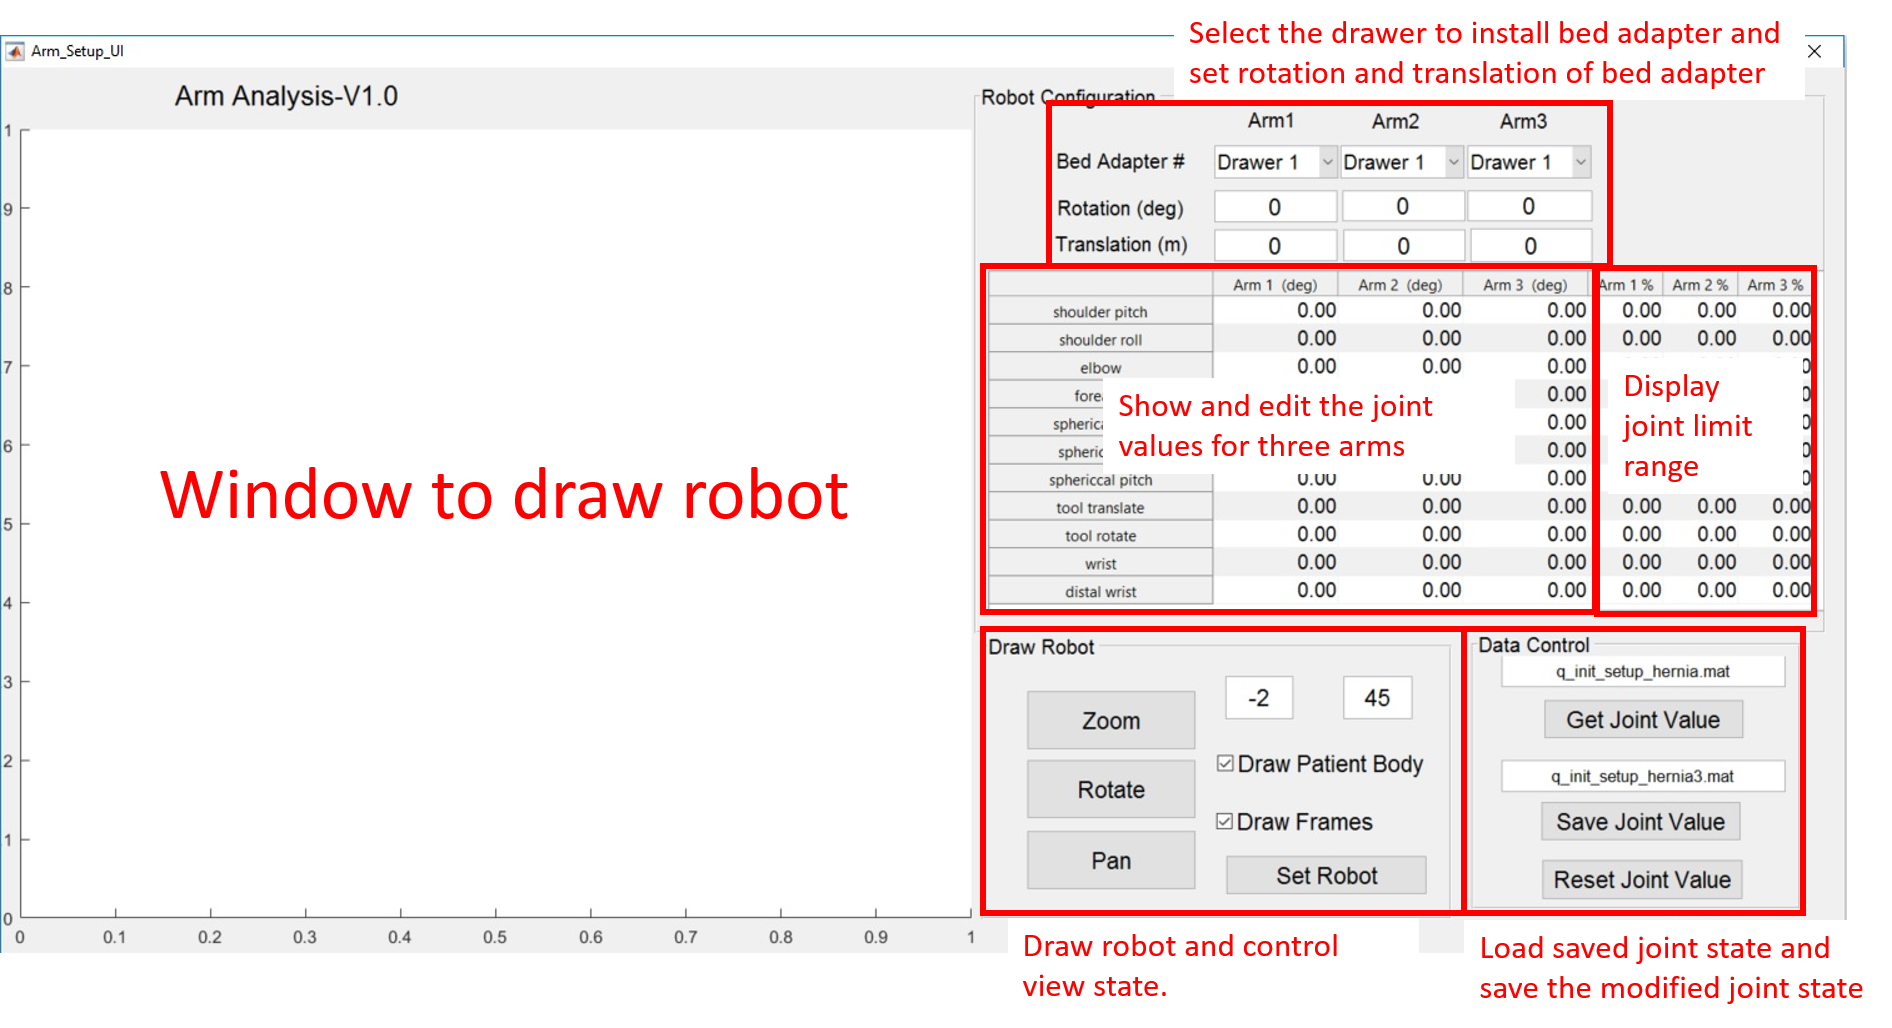
\includegraphics[width=1\columnwidth]{GUI_function}
	\caption{Function blocks of the GUI}\label{fig:GUI_function}
\end{figure}
For Matlab users, please check out the rouxeny/arm\_analysis from github, locate to \textbf{haoran\_model} folder and run \textbf{StartUp.m} to initialize. Then in command window, type \textbf{Arm\_Setup\_UI} to run the GUI. Figure \ref{fig:GUI_function} shows the introduction of the GUI panels. 

In the \textbf{Robot Configuration} panel, the user can select the drawer, change the rotation and translation of table adapter and set all 11 active joints for each arm. The unit for all revolute joints are in degrees and the tool translation is in meters. Column 1 to 3 of the table are joint values and Column 4 to 6 are current joint percentage inside the joint limits (0\% means at lower bound and 100\% means at upper bound). 

In the \textbf{Data Control} panel, user can load existing robot configuration by specifying the file name ("q\_init\_setup\_hernia.mat" for example) and click \textbf{Get Joint Value} to load the robot configuration into the bed adapter and table. Similary, one can also type file name and save all the current values into the specified file. \textbf{Reset Joint Value} will reset all the joint value to 0.

In the  \textbf{Draw Robot} panel, \textbf{Set Robot} will take the values from Robot configuration and draw the robot in display window. User can rotate, zoom and pan like viewing a Matlab figure. Two values in the edit box can set the original view state of the Matlab figure using command view(az,el).

\begin{figure}[htbp]
  \centering
    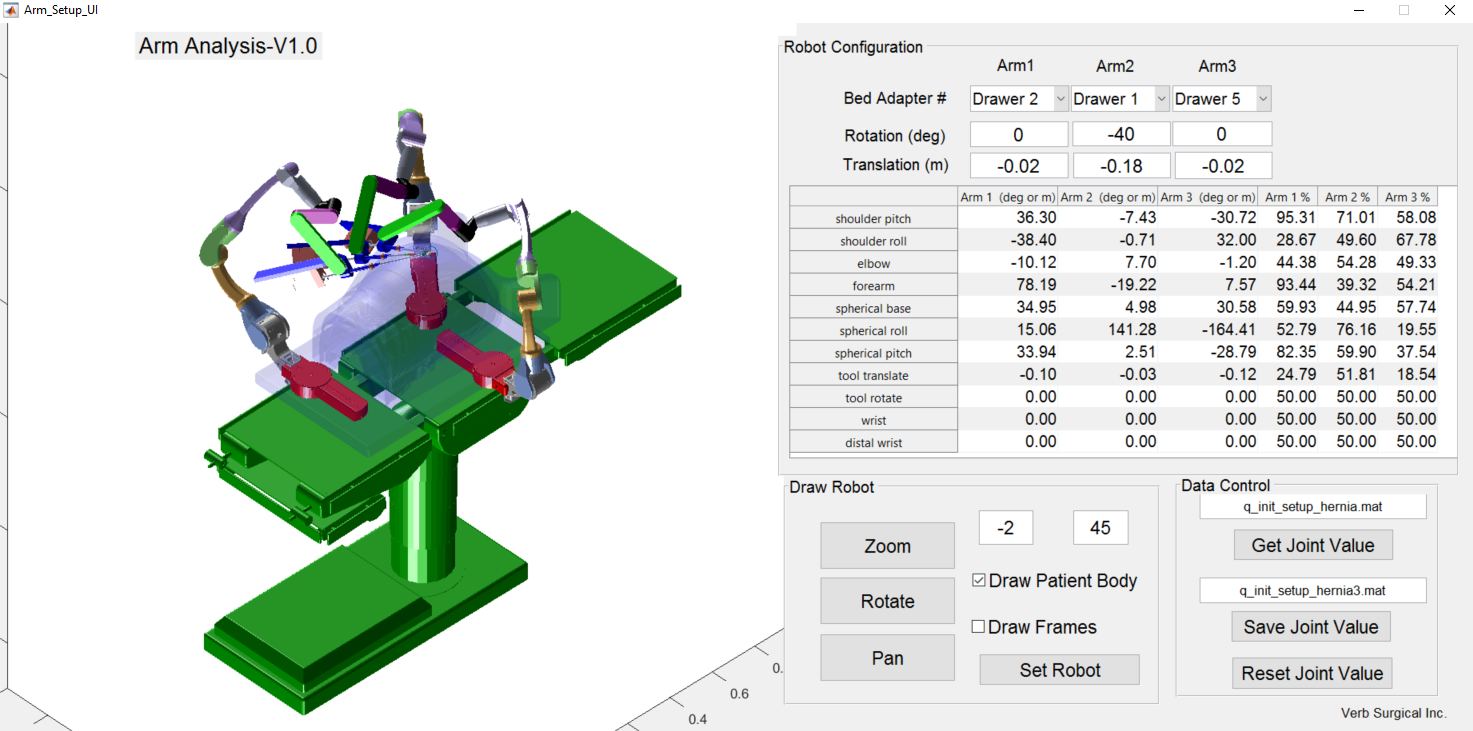
\includegraphics[width=1\columnwidth]{GUI_robot}
	\caption{GUI with the robot}\label{fig:GUI_robot}
\end{figure}
\section{Arm Setup}
The Matlab GUI will help the user visualize the setup and choose an estimated setup. Then the user can open the matlab script "AnalysisHerniaProcedureSetup.m" and load the data file saved from GUI. This script also needs the user to modifiy the file "InitHerniaSetup.m" if the procedure setup such as target region and trocar position change. User can run the script "AnalysisHerniaProcedureSetup.m" to generate the actual robot setup and save it to "file\_name\_you\_choose.mat" by running command

"save('data\textbackslash q\_init\_setup\_hernia.mat','q\_init\_setup','q\_bed\_adapter','selected\_bed\_adapter')"
\section{Future features}
Future features if needed could include:
\begin{enumerate}
\item functionality to run automatic arm setup with given input.
\item load collision analysis data and display.
\item plot other things such as: joint velocity and etc.
\end{enumerate}
\end{document}